\begin{defn}
	Soit $Q \subseteq \mathcal{E} \times \mathcal{S}$\/ un problème.
	Soit $\mathrm{opt} \in \{\min, \max\}$. On dit que $Q$\/ est un \textit{problème d'$\mathrm{opt}$imisation} (\textit{i.e.} problème de minimisation, maximisation), si pour toute entrée $e \in \mathcal{E}$, il existe
	\begin{itemize}
		\item un ensemble $\mathrm{sol}(e)$\/ de solutions,
		\item une fonction $c_e : \mathrm{sol}(e) \to \R^+$,
	\end{itemize}
	tels que $c_e^\star = \mathrm{opt}\{c_e(s)  \mid s \in \mathrm{sol}(e)\}$\/ est bien défini, et \[
		\forall s \in \mathrm{sol}(e),\quad\quad (e, s) \in Q \implies c_e(s) = c_e^\star 
	.\]
	On nomme :
	\begin{itemize}
		\item $\mathrm{sol}(e)$\/ l'\textit{ensemble des solutions pour l'entrée $e$},
		\item $c_e$\/ \textit{la fonction objectif},
		\item $c_e^\star$\/ la \textit{valeur $\mathrm{opt}$imale} (minimale ou maximale),
		\item pour une solution $s \in \mathrm{sol}(e)$, $c_e(s)$\/ est appelée la \textit{valeur de la solution}.
	\end{itemize}
	On appelle \textit{solution $\mathrm{opt}$imale} \ul{une} solution de valeur $\mathrm{opt}$imale.
\end{defn}

\begin{exm}
	On considère le problème \[
		\begin{cases}
			\text{\textbf{Entrée}} &: G = (S, A) \text{ un graphe orienté fortement connexe},\: s \in S, \text{ et } p \in S\\
			\text{\textbf{Sortie}} &: \text{un plus court chemin (en nombre d'arcs) de $s$ à $p$ dans $G$.}
		\end{cases}
	\]
	Soit l'entrée ci-dessous.
	\begin{figure}[H]
		\centering
		\tikzfig{plus-court-chemin}
		\caption{Entrée du problème du plus court chemin}
	\end{figure}
	L'ensemble $\mathrm{sol}(e)$\/ est l'ensemble (infini) des chemins de $s$\/ à $p$, et $c_e(\gamma) = |\gamma|$\/ (la longueur du chemin $\gamma$).
	On vérifie qu'il existe un chemin de $s$\/ à $p$, donc $\{c_e(s)  \mid s \in \mathrm{sol}(e)\} $\/ est une partie de $\N$\/ non vide, elle admet donc un minimum.
\end{exm}

\begin{defn}
	Le \textit{problème de décision associé} à un problème d'$\mathrm{opt}$imisation est le problème obtenu en ajoutant une constante aux entrées et en demandant en sortie s'il est possible de dépasser cette constante.
\end{defn}

\begin{exm}
	Étant donné le problème d'$\mathrm{opt}$imisation \[
		Q_\mathrm{O} : \begin{cases}
			\text{\textbf{Entrée}} &: e \in \mathcal{E}_{Q_\mathrm{O}}\\
			\text{\textbf{Sortie}} &: \mathop{\mathrm{arg\,opt}}_{s \in \mathrm{sol}(e)} c_e(s),
		\end{cases}
	\]
	on définit le problème de décision associé
	\[
		Q : \begin{cases}
			\text{\textbf{Entrée}} &: e \in \mathcal{E}_{Q_\mathrm{O}},\: K \in \R^+\\
			\text{\textbf{Sortie}} &: \text{existe-t-il } s \in \mathrm{sol}(e) \text{ tel que } c_e(s) \mathrel{\bowtie} K
		\end{cases}
	\] avec ${\bowtie} = {\le}$\/ si $\mathrm{opt} = {\min}$ et ${\bowtie} = {\ge}$\/ si $\mathrm{opt} = {\max}$.
\end{exm}

\begin{exm}
	Avec l'exemple précédent (plus court chemin), le problème de décision associé est \[
		\begin{cases}
			\text{\textbf{Entrée}} &: G = (S, A) \text{ un graphe orienté fortement connexe},\: (p, s) \in S^2, \text{ et } K \in \R^+\\
			\text{\textbf{Sortie}} &: \text{Existe-t-il un chemin de $s$\/ à $p$\/ dans $G$\/ de longueur inférieure ou égale à $K$\/ ?}
		\end{cases}
	\]
\end{exm}

\begin{exm}
	On considère le problème \textsc{Knapsack} de décision défini comme \[
		\begin{cases}
			\text{\textbf{Entrée}} &: \text{Un entier } n \in \N,\:(p_1, \ldots, p_n) \in (\N^*)^n,\:(v_1, \ldots, v_n) \in (\N^*)^n,\: P \in \N \text{ et } K \in \N\\
			\text{\textbf{Sortie}} &: \text{Existe-t-il $I \subseteq \llbracket 1,n \rrbracket$\/ telle que $\sum_{i \in I} p_i \le P$\/ et $\sum_{i \in I} v_i \ge K$\/ ?}
		\end{cases}
	\] Le problème d'$\mathrm{opt}$imisation associé est \textsc{Knapsack}$_\mathrm{O}$ défini comme \[
		\begin{cases}
			\text{\textbf{Entrée}} &: \text{Un entier } n \in \N,\:(p_1, \ldots, p_n) \in (\N^*)^n,\:(v_1, \ldots, v_n) \in (\N^*)^n, \text{ et }P \in \N\\
			\text{\textbf{Sortie}} &: I \subseteq \llbracket 1,n \rrbracket \text{ tel que } \sum_{i \in I} p_i \le P \text{ et maximisant } \sum_{i \in I} v_i.
		\end{cases}
	\]
\end{exm}

\begin{rmk}
	Soit $Q_\mathrm{O}$\/ un problème d'$\mathrm{opt}$imisation et $Q$\/ le problème de décision associé.
	Étant donné un algorithme $\mathcal{A}_\mathrm{O}$ pour $Q_\mathrm{O}$, on fabrique l'algorithme $\mathcal{A}$\/ suivant résolvant $Q$.
	\begin{algorithm}[H]
		\centering
		\begin{algorithmic}[1]
			\Entree $e$\/ une entrée de $Q_\mathrm{O}$\/ et $K$\/ un seuil
			\State\Return $\ds c_e(\mathcal{A}_\mathrm{O}) \mathrel{\mathop{\bowtie}^?} K$
			\Comment{où $\bowtie$ est $\ge$\/ pour si $\mathrm{opt}$\/ est $\max$, et $\le$\/ si $\mathrm{opt}$\/ est $\min$}
		\end{algorithmic}
		\caption{Solution à un problème de seuil}
	\end{algorithm}
	Ainsi, le problème $Q_\mathrm{O}$\/ est plus difficile à résoudre que le problème $Q$\/ de décision associé. Alors, lorsque le problème de décision $Q$\/ associé à un problème d'$\mathrm{opt}$imisation $S_\mathrm{O}$\/ est \textbf{NP}-difficile, c'est mal engagé.
\end{rmk}

\section{Algorithmes d'approximations}

\begin{rmk}[Vocabulaire]
	On fixe dans la suite un problème d'$\mathrm{opt}$imisation $Q$, on note $\mathrm{OPT}(e)$\/ la valeur $\mathrm{opt}$imale pour une entrée $e$.
\end{rmk}

\begin{defn}[Algorithme d'approximation pour un problème de maximisation]
	On dit d'un algorithme $\mathcal{A} : \mathcal{E}_Q \to \R^+$\/ qu'il approxime un problème $Q$\/ de maximisation avec un ratio d'approximation $\rho < 1$\/ dès lors que \[
		\forall e \in \mathcal{E}_Q, \quad \mathcal{A}(e) \ge \rho \cdot \mathrm{OPT}(e)
	.\]
	On dit alors que l'algorithme $\mathcal{A}$\/ est une \textit{$\rho$-approximation} (standard).
\end{defn}

\begin{figure}[H]
	\centering
	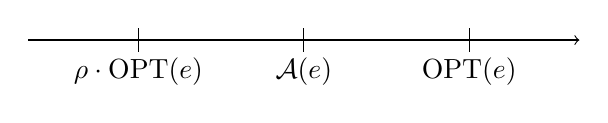
\begin{tikzpicture}[yscale=0.2,xscale=0.7]
		\draw[->] (0,0) -- (10, 0);
		\draw (2,-0.75)--(2,0.75); \node at (2, -2) {$\rho \cdot \mathrm{OPT}(e)$};
		\draw (5,-0.75)--(5,0.75); \node at (5, -2) {$\mathcal{A}(e)$};
		\draw (8,-0.75)--(8,0.75); \node at (8, -2) {$\mathrm{OPT}(e)$};
	\end{tikzpicture}
	\caption{Algorithme d'approximation pour un problème de maximisation}
\end{figure}

\begin{defn}[Algorithme d'approximation pour un problème de minimisation]
	On dit d'un algorithme $\mathcal{A} : \mathcal{E}_Q \to \R^+$\/ qu'il approxime un problème $Q$\/ de minimisation avec un ratio d'approximation $\rho > 1$\/ dès lors que \[
		\forall e \in \mathcal{E}_Q, \quad \mathcal{A}(e) \le \rho \cdot \mathrm{OPT}(e)
	.\]
	On dit alors que l'algorithme $\mathcal{A}$\/ est une \textit{$\rho$-approximation} (standard).
\end{defn}

\begin{figure}[H]
	\centering
	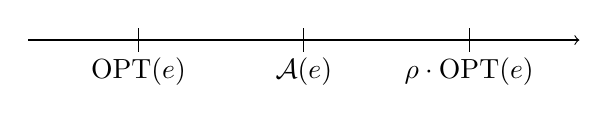
\begin{tikzpicture}[yscale=0.2,xscale=0.7]
		\draw[->] (0,0) -- (10, 0);
		\draw (2,-0.75)--(2,0.75); \node at (2, -2) {$\mathrm{OPT}(e)$};
		\draw (5,-0.75)--(5,0.75); \node at (5, -2) {$\mathcal{A}(e)$};
		\draw (8,-0.75)--(8,0.75); \node at (8, -2) {$\rho \cdot \mathrm{OPT}(e)$};
	\end{tikzpicture}
	\caption{Algorithme d'approximation pour un problème de minimisation}
\end{figure}

Dans la définition suivante, on suppose connu une fonction $\mathrm{Pire}(e)$\/ donnant la pire valeur de solution pour une entrée $e$.
\begin{defn}
	On dit qu'un algorithme $\mathcal{A} : \mathcal{E}_Q \to \R$\/ est une \textit{$\rho$-approximation différentielle} dès lors que \[
		\frac{\big|\mathcal{A}(e) - \mathrm{Pire}(e)\big|}{\big|\mathrm{Pire}(e) - \mathrm{OPT}(e)\big|} \ge \rho
	.\]
\end{defn}

\begin{figure}[H]
	\centering
	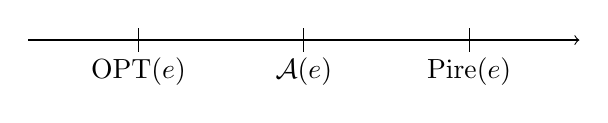
\begin{tikzpicture}[yscale=0.2,xscale=0.7]
		\draw[->] (0,0) -- (10, 0);
		\draw (2,-0.75)--(2,0.75); \node at (2, -2) {$\mathrm{OPT}(e)$};
		\draw (5,-0.75)--(5,0.75); \node at (5, -2) {$\mathcal{A}(e)$};
		\draw (8,-0.75)--(8,0.75); \node at (8, -2) {$\mathrm{Pire}(e)$};
	\end{tikzpicture}
	\caption{$\rho$-approximation différentielle}
\end{figure}

\begin{rmk}
	Dans le cadre d'un problème de minimisation, on ne calcule pas $\mathrm{OPT}(e)$\/ en général. On minore $\mathrm{OPT}(e)$, et alors \[
		\frac{\mathcal{A}(e)}{\mathrm{OPT}(e)} \le \underbrace{\frac{\mathcal{A}(e)}{B}}_{\rho}
	.\]
\end{rmk}

\begin{figure}[H]
	\centering
	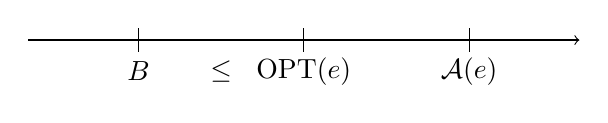
\begin{tikzpicture}[yscale=0.2,xscale=0.7]
		\draw[->] (0,0) -- (10, 0);
		\draw (2,-0.75)--(2,0.75); \node at (2, -2) {$B$};
		\draw (5,-0.75)--(5,0.75); \node at (5, -2) {$\mathrm{OPT}(e)$};
		\draw (8,-0.75)--(8,0.75); \node at (8, -2) {$\mathcal{A}(e)$};
		\node at (3.5, -2) {$\le$};
	\end{tikzpicture}
	\caption{Calcul de $\mathrm{OPT}(e)$}
\end{figure}

\begin{exm}
	Soit $C \in \N^*$.
	On rappelle le problème \textsc{Stable}, restreint à un graphe de degré maximal $C$\/ : \[
		\textsc{Stable} : \begin{cases}
			\text{\textbf{Entrée}} &: G = (S, A) \text{ une graphe tel que } 0 \neq \Delta(G) \le C\\
			\text{\textbf{Sortie}} &: \text{ un stable de $G$\/ de cardinal maximal}
		\end{cases}
	\]
	où $X\subseteq S$\/ est un stable si pour tout $(u,v) \in X^2$, $\{u,v\} \not\in A$, et $\Delta(G) = \max_{v \in S} \deg_G(v)$ est le degré du graphe.
\end{exm}

\begin{algorithm}[H]
	\centering
	\begin{algorithmic}[1]
		\Entree $G = (S, A)$\/ un graphe
		\State $S' \gets \O$\/ 
		\While {$S \neq \O$}
			\State $v^\star = \argmin_{v \in S} \deg_G(v)$\/  \Comment{les degrés sont modifiés à chaque itération}
			\State $S' \gets S' \cup \{v^\star\}$\/
			\State $S \gets S \setminus \big(\{v^\star\} \cup \mathrm{voisins}(v^\star)\big)$\/
			\State $A \gets \text{ restriction de $A$ à $S$}$\/
		\EndWhile
		\State\Return $S'$\/
	\end{algorithmic}
	\caption{Algorithme glouton de recherche de stables}
	\label{algo:recherche-de-stable-glouton}
\end{algorithm}

Cet algorithme n'est pas correct, la figure ci-après en est un contre-exemple.

\begin{figure}[H]
	\centering
	\begin{tikzpicture}
		\node[style=new style 0] (A0) at (0, 0) {};
		\node[style=new style 0] (A1) at (1, 0) {};
		\node[style=new style 0] (A2) at (0, 1) {};
		\node[style=new style 0] (A3) at (1, 1) {};
		\node[style=new style 0] (A4) at (2, 1) {};
		\node[style=new style 0] (A5) at (1, 2) {};
		\node[style=new style 0] (A6) at (2, 2) {};
		\node[style=new style 0] (A7) at (3, 2) {};
		\node[style=new style 0] (A8) at (2, 3) {};
		\node[style=new style 0] (A9) at (3, 3) {};
		\draw (A0) -- (A1) (A0) -- (A2) (A1) -- (A3) (A2) -- (A3);
		\draw (A3) -- (A4) (A3) -- (A5) (A5) -- (A6) (A4) -- (A6);
		\draw (A6) -- (A7) (A6) -- (A8) (A7) -- (A9) (A8) -- (A9);
	\end{tikzpicture}
	\begin{comment}
		0-1
		| |
		2-3-4
		  | |
			5-6-7
			  | |
				8-9
	\end{comment}
	\caption{Contre-exemple à l'algorithme \ref{algo:recherche-de-stable-glouton}}
\end{figure}

\begin{prop}
	L'algorithme \ref{algo:recherche-de-stable-glouton} est une $\frac{1}{\Delta(G)}$-approximation.
\end{prop}

\begin{prv}
	Soit $S'$\/ la réponse de l'algorithme.
	Soit $S^\star$\/ la solution optimale.
	On a, par terminaison de l'algorithme \[
		\forall v \in S \setminus S, \exists v' \in S',\: \{v,v'\} \in A
	\] car l'algorithme s'arrête. En particulier, $\forall v^\star \in S^\star \setminus S',\:\exists v' \in S',\: \{v, v'\} \in A$.
	Or, $S^\star$\/ est stable donc, si $v^\star\in S^\star$ et $v' \in S'$ tels que $\{v^\star, v' \in A\}$, alors $v' \not\in S^\star$. D'où, \[
		\forall v^\star \in S^\star \setminus S',\: \exists v' \in S' \setminus S^\star,\: \{v^\star, v'\} \in A
	.\]
	Par définition de degré d'un graphe, on a $|S^\star \setminus S'| \le \Delta(G) \:|S' \setminus S^\star|$\/ donc
	\begin{align*}
		|S^\star| &= |S^\star \cap S'| + |S^\star \setminus S'| \\
		&\le  |S^\star \cap S'| + \Delta(G)\:|S' \setminus S^\star|\\
		&\le \Delta(G)\:|S^\star  \cap S'| + \Delta(G)\:|S' \setminus S^\star|\\
		&\le \Delta(G) \:|S'|.
	\end{align*}
\end{prv}
